\documentclass[a4paper,12pt]{article}
\usepackage{../../mypackages}
\usepackage{../../macros}
\usepackage{array,multirow}
\usepackage[table]{xcolor}  % Load xcolor with the table option for colored cells
\usepackage{colortbl}       % Load colortbl for \columncolor in tables

\usepackage{pgfplots}
    \pgfplotsset{
    compat=1.11,
  }

\setlength{\parindent}{0pt}

\begin{document}

\title{Méthodes - 3ème - Physique Chimie}
\author{N. Bancel}

\maketitle
\def\WITH_CORRECTION{YES}

\section{Les unités du système international}

\begin{figure}[H]
  \centering
  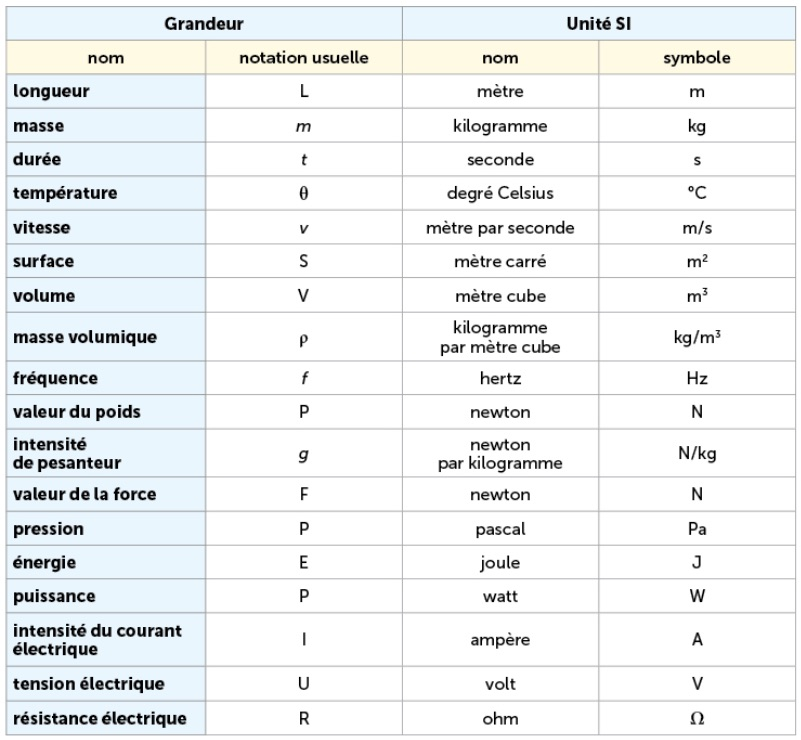
\includegraphics[width=0.7\linewidth]{unites.jpg}
\end{figure}

\section{Multiples et sous multiples}

\begingroup
\renewcommand{\arraystretch}{1.5}
%\setlength{\tabcolsep}{6pt}

\begin{center}
  \begin{tabularx}{\linewidth}{|>{\columncolor{cyan!10}}c |>{\columncolor{cyan!10}}c |>{\columncolor{cyan!10}}c |>{\columncolor{cyan!10}}c |>{\columncolor{cyan!10}}c |>{\columncolor{cyan!10}}c |>{\columncolor{cyan!10}}c |>{\columncolor{yellow!20}}c |>{\columncolor{green!10}}c |>{\columncolor{green!10}}c |>{\columncolor{green!10}}c |>{\columncolor{green!10}}c |>{\columncolor{green!10}}c |}
      \hline
      $10^{-15}$ & $10^{-12}$ & $10^{-9}$ & $10^{-6}$ & $10^{-3}$ & $10^{-2}$ & $10^{-1}$ & $1$ & $10^{1}$ & $10^{2}$ & $10^{3}$ & $10^{6}$ & $10^{9}$ \\ 
      \hline
      f & p & n & $\mu$ & m & c & d & -- & da & h & k & M & G \\
      \hline
      femto & pico & nano & micro & milli & centi & déci & -- & déca & hecto & kilo & méga & giga \\
      \hline
  \end{tabularx}
  \end{center}
  \endgroup

  \subsection{Conversions avec puissances}

\textcolor{blue}{\textbf{Exemples de conversions}}
\vspace{1em}

Pour convertir \SI{4.6e05}{mL} en $L$, on suit les étapes suivantes :

1. \textbf{Relation entre mL et L} :

Donc $1 \text{L} = 1000 \text{mL} = 10^3 \, \text{mL}$.
Et $1 \text{mL} = \frac{1}{10^3} \text{L}$

2. \textbf{Écrire la conversion et appliquer les formules de puissances} : 
   \[
    \SI{4.6e5}{mL} = \frac{\num{4.6e5}}{10^3}~\si{L}
   = 4.6 \times 10^{5-3}~\si{L}
   = \num{4.6e02}~\si{L}
   \]

\textcolor{blue}{\textbf{Exercice}}

\vspace{1em}

\begin{tabularx}{\textwidth}{>{\raggedright\arraybackslash}X >{\raggedright\arraybackslash}X}
  \toprule
  \textbf{Conversion} & \textbf{Réponse} \\
  \midrule
  Convertir \SI{5}{km} en mètres & \trou{$5 \times 10^3 ~\si{m} = 5000 ~\si{m}$}{\ndots[20]} \\
  \midrule
  Convertir \SI{3.5e03}{g} en kilogrammes & \trou{$1 g = 10^{-3} ~kg$ donc : $3.5 \times 10^3 \times 10^{-3} = 3.5 ~kg$}{\ndots[20]} \\
  \midrule
  Convertir \SI{2.5}{L} en millilitres & {\trou{$1~L = 10^3~mL$ donc $2.5 \times 10^3~mL$}{\ndots[20]}} \\
  \midrule
  Convertir \SI{4.6e5}{mL} en litres & {\trou{\SI{460}{L}}{\ndots[20]}} \\
  \midrule
  Convertir \SI{0.75}{kg} en grammes & {\trou{\SI{750}{g}}{\ndots[20]}} \\
  \midrule
  Convertir \SI{1.2e6}{mg} en kilogrammes & {\trou{\SI{1.2}{kg}}{\ndots[20]}} \\
  \midrule
  Convertir \SI{0.034}{km} en centimètres & {\trou{\SI{3400}{cm}}{\ndots[20]}} \\
  \bottomrule
\end{tabularx}

\subsection{Conversions avec tableau}

\begin{itemize}[noitemsep]
\item \href{https://v3.globalcube.net/clients/larecre/content/medias/telechargements/mathematique/tableau_mesures_volumes.pdf}{Le tableau des mesures de volume}
\item \href{https://www.cmath.fr/CM2/conversions/cours.php}{Autre type de conversion}
\end{itemize}

\subsection{Conversion d'unités sous forme de fractions}

\subsubsection{Méthode générale}

\begin{tcolorbox}[colback=red!10!white, colframe=red!75!black, title=PAR COEUR]
  Il suffit d'écrire la valeur sous la forme d'une vraie fraction. Et de convertir individuellement chaque élément de la fraction (le numérateur, puis le dénominateur)
\end{tcolorbox}

\subsubsection{Conversion de \si{g/L} en \si{kg/dm^3}}

\textcolor{blue}{\textbf{Exemple : Convertir \SI{500}{g/L} en \si{kg/dm^3}}}

\vspace{1em}
\textbf{Solution} :
\vspace{1em}
On sait que :
\[
\SI{1}{g/L} = \frac{\si{1}{g}}{\si{1}{L}}
\]
Or, \SI{1}{L} est équivalent à \SI{1}{dm^3}, et \SI{1}{g} est équivalent à \SI{e-3}{kg}. Ainsi,
\[
  \SI{1}{g/L} = \frac{\SI{e-3}{kg}}{\SI{1}{dm^3}} = \SI{1e-3}{kg/dm^3}
\]
Par conséquent :
\[
500 \, \si{g/L} = 5 \times 10^2 \times \SI{1e-3}{kg/dm^3} = \SI{5e-1}{kg/dm^3}
\]

\subsubsection{Conversion de \si{m/s} en \si{km/h}}

\textcolor{blue}{\textbf{Exemple : Convertir \SI{15}{m/s} en \si{\km/h}.}}

\vspace{1em}

\textbf{Solution} : On sait que : \\

\[
1 \, \si{m/s} = \frac{1 \, \si{m}}{1 \, \si{s}}
\]
Or, 
\[
1 m = \frac{1}{1000} km \quad \text{et} \quad 1 s = \frac{1}{3600} h 
\]
On a donc :
\[
  \SI{1}{m/s} = \frac{1}{1000 \times \frac{1}{3600}} \text{km/h} = \frac{3600}{1000} \text{km/h} = \SI{3.6}{km/h}
\]
Ainsi :
\[
  \SI{15}{m/s} = 15 \times 3.6 ~\text{km/h} = \SI{54}{km/h}
\]


\section{Précision d'une mesure}

Un appareil mesure une valeur avec un certain degré d'imprécision. C'est-à-dire qu'en lisant la valeur, on ne peut pas être certain qu'elle est parfaitement exacte : on précise donc un intervalle entre lequel on pense que la valeur réelle se situe. 

\subsection{Précision d'une mesure - Partie 1}

\textcolor{blue}{\textbf{Exemple}} 
\vspace{1em}

\textbf{Vérification de l’hypothèse selon laquelle la masse se conserverait lors de la fusion d’un glaçon avec une balance de précision $\pm 0,2$ g.}

\begin{figure}[H]
  \centering
  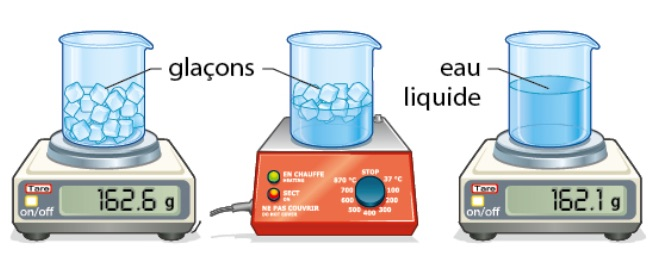
\includegraphics[width=0.7\linewidth]{balances.jpg}
\end{figure}

\begin{enumerate}[noitemsep]
    \item $m_{\text{avant}} = 162,6 \pm 0,2$ g. La masse est comprise entre 162,4 g et 162,8 g.
    \item $m_{\text{après}} = 162,1 \pm 0,2$ g. La masse est comprise entre \SI{162,1}{g} et \SI{162,3}{g}.
\end{enumerate}


\begin{figure}[H]
  \centering
  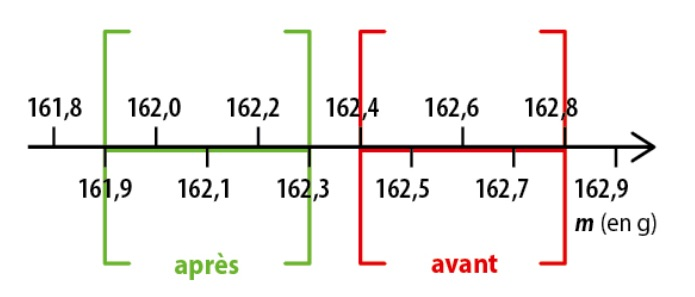
\includegraphics[width=0.7\linewidth]{intervalles_balances.jpg}
  \caption{Représentation des intervalles}
\end{figure}

Les intervalles ne se chevauchent pas. On ne peut pas conclure que la masse se conserve lors de la fusion.
Avant d'invalider l'hypothèse, il faut s'interroger sur la pertinence du protocole suivi.

\vspace{1em}

Ici, on pourrait penser que de l'eau s'est évaporée lors du chauffage. Il convient alors de refaire l'expérience en choisissant un récipient fermé.

\subsection{Précision d'une mesure - Partie 2 (avec des pourcentages)}


\textcolor{blue}{\textbf{Exemple}}

\vspace{1em}

\textbf{Vérification de l’hypothèse selon laquelle l’intensité du courant électrique diminuerait dans un circuit en série, avec un ampèremètre de précision égale à $\pm (0.3 \, \% \times I + 0.01 \, \text{A})$.} $I$ est la valeur affichée par l’ampèremètre.

\begin{figure}[H]
  \centering
  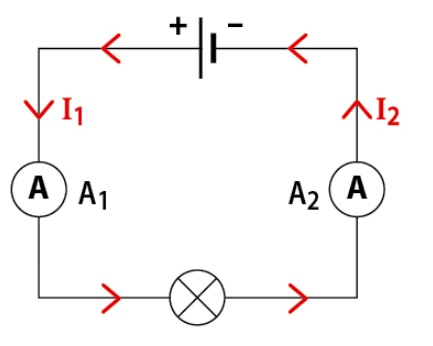
\includegraphics[width=0.7\linewidth]{circuit.jpg}
\end{figure}

\begin{itemize}[noitemsep]
    \item Lors de la mesure de $I_1$, l’ampèremètre affiche 0,23 A.
    La précision de cette mesure se calcule donc comme suit :
    $0,3 \, \% \times I + 0,01 \, \text{A} = \frac{3}{100} \times 0,23 \, \text{A} + 0,01 \, \text{A} = 0,017 \, \text{A}$.
    
    \item On arrondit le résultat au centième supérieur.
    Cela donne donc une précision égale à 0,02 A.
    Le résultat de la mesure de $I_1$ s’écrit \textbf{$I_1 = 0,23 \pm 0,02 \, \text{A}$}.
    
    \item Lors de la mesure de $I_2$, l’ampèremètre affiche 0,22 A.
    De la même manière, \textbf{$I_2 = 0,22 \pm 0,02 \, \text{A}$}.
\end{itemize}


\begin{figure}[H]
  \centering
  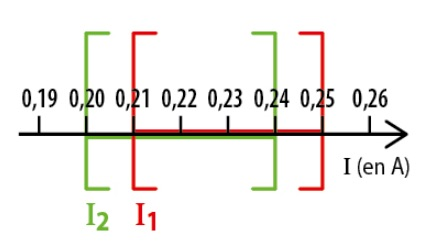
\includegraphics[width=0.7\linewidth]{circuite_intervalles.jpg}
  \caption{Représentation des intervalles}
\end{figure}

Les intervalles se chevauchent. On peut donc en conclure que l’intensité n’est pas plus faible après la lampe qu’avant.

\vspace{1em}

Pour conclure que l’intensité du courant électrique ne varie pas dans un circuit en série, il faudrait reproduire l’expérience un grand nombre de fois, en exploitant les résultats de tous les groupes de la classe et vérifier si les intervalles se chevauchent dans chaque groupe.


\section{La notation scientifique et les chiffres significatifs}

\subsection{Notation scientifique}

\begin{tcolorbox}[colback=red!10!white, colframe=red!75!black, title=PAR COEUR]
  La notation scientifique permet de représenter des nombres très grands ou très petits de manière simplifiée. Un nombre est exprimé sous la forme :
\[
N = a \times 10^n
\]
où :
\begin{itemize}[noitemsep]
    \item \( a \) est un nombre réel tel que \( 1 \leq |a| < 10 \),
    \item \( n \) est un entier relatif (positif ou négatif).
\end{itemize}
\end{tcolorbox}

\textbf{Exemple} : Le nombre \( 123000 \) peut être écrit comme \( 1,23 \times 10^5 \). \\

\textcolor{blue}{\textbf{Exercice}} : Ecris les nombres suivants en notation scientifique
\vspace{1em}

\begin{tabularx}{8cm}{| >{\raggedright\arraybackslash}p{3cm} | >{\raggedright\arraybackslash}X |} 
  \toprule
  {\textbf{Nombre}} & {\textbf{Notation scientifique}} \\
  \midrule
  {45000} & {\trou{$4,5 \times 10^4$}{\ndots[20]}} \\
  \midrule
  {0,00032} & {\trou{$3,2 \times 10^{-4}$}{\ndots[20]}} \\
  \midrule
  {7250000} & {\trou{$7,25 \times 10^6$}{\ndots[20]}} \\
  \midrule
  {0,00000056} & {\trou{$5,6 \times 10^{-7}$}{\ndots[20]}} \\
  \midrule
  {120} & {\trou{$1,2 \times 10^2$}{\ndots[20]}} \\
  \midrule
  {502300} & {\trou{$5,023 \times 10^5$}{\ndots[20]}} \\
  \midrule
  {0,00000789} & {\trou{$7,89 \times 10^{-6}$}{\ndots[20]}} \\
  \bottomrule
\end{tabularx}



\subsection{Chiffres significatifs}



Les chiffres significatifs représentent la précision d'une mesure ou d'un calcul. Voici quelques règles pour les identifier :
\begin{itemize}[noitemsep]
    \item Les zéros situés entre deux chiffres significatifs sont significatifs.
    \item Les zéros situés à gauche d’un nombre ne sont pas significatifs.
    \item Les zéros à la droite d'un nombre décimal sont significatifs.
    \item \textbf{Dans le cas de la notation scientifique, seuls les chiffres avant le x 10 sont significatifs}
\end{itemize}

\begin{tcolorbox}[colback=gray!10!white, colframe=gray!75!black, title=Autrement dit]
  Tous les chiffres sont significatifs sauf les 0 "écrits à gauche"
\end{tcolorbox}

\begin{tcolorbox}[colback=green!10!white, colframe=green!75!black, title=Interprétation]
  Les chiffres significatifs sont les chiffres d'un nombre qui expriment la précision d'une mesure. \\

  \vspace{1em}

  Imaginons une balance de cuisine qui affiche "100,0 g" pour un objet. \\

  \vspace{1em}

  La balance indique ici quatre chiffres significatifs, ce qui montre qu'elle mesure jusqu'au dixième de gramme.
  Si une autre balance affiche "100 g", cela signifie qu'elle est moins précise, ne mesurant qu'à l'unité de gramme près.
  
  \vspace{1em}

  Les chiffres significatifs représentent donc le niveau de détail de la mesure, et nous devons en tenir compte pour ne pas surestimer la précision d'un instrument de mesure.

\end{tcolorbox}

\textbf{Exemple} : Dans \( 0,00560 \), il y a trois chiffres significatifs : \( 5 \), \( 6 \) et le dernier zéro.

\vspace{1em}

\begin{tabularx}{\textwidth}{>{\raggedright\arraybackslash}p{3cm} >{\raggedright\arraybackslash}X}
  \toprule
  {\textbf{Nombre}} & {\textbf{Nombre de chiffres significatifs}} \\
  \midrule
  {0,0450} & {\trou{3 chiffres significatifs (4, 5 et le dernier 0 après le point décimal)}{\ndots[20]}} \\
  \midrule
  {3,200} & {\trou{4 chiffres significatifs (3, 2, 0, et 0, car les zéros à droite d'un nombre décimal sont significatifs).}{\ndots[20]}} \\
  \midrule
  {500} & {\trou{1 chiffre significatif (le 5, car les zéros à droite sans point décimal ne sont pas significatifs)}{\ndots[20]}} \\
  \midrule
  {0,0032} & {\trou{2 chiffres significatifs (3 et 2 ; les zéros à gauche ne sont pas significatifs)}{\ndots[20]}} \\
  \midrule
  {7,0000} & {\trou{5 chiffres significatifs (7 et les quatre zéros après la virgule).}{\ndots[20]}} \\
  \midrule
  {123,45} & {\trou{5 chiffres significatifs (tous les chiffres sont significatifs dans ce nombre)}{\ndots[20]}} \\
  \midrule
  {$6,02 \times 10^{23}$} & {\trou{3 chiffres significatifs (6, 0, et 2 ; en notation scientifique, seuls les chiffres avant le x10 sont significatifs)}{\ndots[20]}} \\
  \bottomrule
\end{tabularx}

% {l l l}
\begin{tabularx}{\textwidth}{>{\raggedright\arraybackslash}X >{\raggedright\arraybackslash}X >{\raggedright\arraybackslash}X}
  \toprule
  {\textbf{Règle}} & {\textbf{Précision}} & {\textbf{Exemples}} \\
  \midrule
  {Tous les chiffres différents de zéro sont significatifs.}
  & \multirow{2}{=}{Pour déterminer le nombre de chiffres significatifs, il suffit de compter le nombre de chiffres que comporte le nombre.}
  & {e nombre 9,56 possède 3 chiffres significatifs. Le nombre 456,5687 possède 7 chiffres significatifs.} \\
  
    {Tous les zéros situés entre des chiffres différents de zéro sont significatifs.}
    &  
    & {Le nombre 4507 possède 4 chiffres significatifs. Le nombre 40,56 possède 4 chiffres significatifs.} \\
    \midrule
  {Les zéros situés au début d'un nombre ne sont pas significatifs.}
  &
  {Pour déterminer le nombre de chiffres significatifs, il faut repérer le premier chiffre différent de 0 et compter le nombre de chiffres à droite de ce 0.}
  &
  {Le nombre 0,0056 possède 2 chiffres significatifs. Le nombre 0,956 possède 3 chiffres significatifs.} \\ 
  \midrule

  {Tous les zéros situés à la fin d'un nombre décimal sont significatifs.}
    & {Pour déterminer le nombre de chiffres significatifs, il faut compter les chiffres que comporte le nombre (tout en excluant les zéros se situant au début du nombre).}
    & {Le nombre \( 0,50600 \) possède 5 chiffres significatifs.} \\
  
    \midrule
  
  {En fonction du contexte, les zéros situés à la fin d’un nombre entier peuvent être significatifs ou non.}
    & {Pour déterminer le nombre de chiffres significatifs, il faut se fier au contexte, par exemple à la précision de l’instrument.}
    & {Si la valeur \( 23\,700 \) est mesurée à l'aide d'un instrument précis à l'unité près, alors \( 23\,700 \) comprend 5 chiffres significatifs. Si la valeur \( 23\,700 \) est mesurée à l'aide d'un instrument précis à la centaine près, alors \( 23\,700 \) comprend 3 chiffres significatifs. On peut donc dire que \( 23\,700 \) est équivalent à \( 2,37 \times 10^4 \)} \\
  
  \midrule

  {Dans une notation scientifique, les chiffres devant la puissance de 10 sont significatifs.}
    & {Pour déterminer le nombre de chiffres significatifs, il faut compter le nombre de chiffres situés à gauche de la puissance de 10.}
    & {Le nombre \( 9,568 \times 10^3 \) possède 4 chiffres significatifs. Le nombre \( 2,5 \times 10^{-2} \) possède 2 chiffres significatifs.} \\

  \bottomrule
\end{tabularx}

\subsection{Précision des mesures et chiffres significatifs}

\begin{tcolorbox}[colback=red!10!white, colframe=red!75!black, title=PAR COEUR]
  Lorsque l’on additionne, soustrait, multiplie, divise des données, le résultat doit toujours être exprimé avec la même précision que \textbf{la valeur la moins précise, soit celle ayant le moins de chiffres significatifs}.
\end{tcolorbox}

\begin{figure}[H]
  \centering
  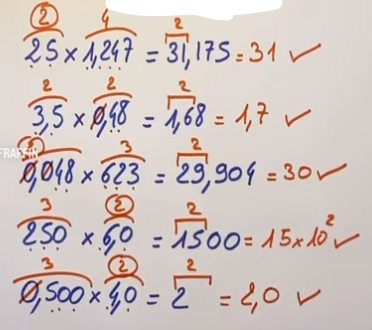
\includegraphics[width=0.7\linewidth]{chiffres_significatifs.jpg}
  \caption{\label{} Chiffres Significatifs}
\end{figure}


\subsection{Vidéos intéressantes - Pour s'entraîner}

\begin{itemize}[noitemsep]
  \item \href{https://www.youtube.com/watch?v=1zAPfrZaAiA&ab_channel=PaulOlivier}{Combien de chiffres significatifs - Paul Olivier}
  \item \href{https://www.youtube.com/watch?v=aJKvYiGXqoM&ab_channel=FlorenceRAFFINlaphysiquechimieaulyc%C3%A9e}{Nombre de chiffres significatifs}
  \item \href{https://youtube.com/shorts/7wfK1r2kft4?si=ufaaWyjVTLT19Iv4}{Nombre de chiffres significatifs - Exercices}
\end{itemize}


\section{Notions mathématiques d'opérations sur les puissances}

Pour manipuler des puissances de 10 et effectuer des calculs plus facilement, voici quelques rappels importants :

\subsection{Multiplication de puissances de même base}
\[
a^m \times a^n = a^{m + n}
\]
\textbf{Exemple} : \( 10^3 \times 10^2 = 10^{3+2} = 10^5 \).

\subsection{Division de puissances de même base}
\[
\frac{a^m}{a^n} = a^{m - n}
\]
\textbf{Exemple} : \( \frac{10^5}{10^3} = 10^{5-3} = 10^2 \).

\subsection{Puissance d'une puissance}
\[
(a^m)^n = a^{m \times n}
\]
\textbf{Exemple} : \( (10^2)^3 = 10^{2 \times 3} = 10^6 \).

\subsection{Puissance de produit}
\[
(a \times b)^n = a^n \times b^n
\]
\textbf{Exemple} : \( (2 \times 5)^3 = 2^3 \times 5^3 = 8 \times 125 = 1000 \).

\subsection{Puissance de quotient}
\[
\left(\frac{a}{b}\right)^n = \frac{a^n}{b^n}
\]
\textbf{Exemple} : \( \left(\frac{4}{2}\right)^2 = \frac{4^2}{2^2} = \frac{16}{4} = 4 \).

\subsection{Puissance de 10}
La puissance de 10 est souvent utilisée pour exprimer des valeurs très grandes ou très petites :
\begin{itemize}[noitemsep]
    \item \( 10^3 = 1000 \),
    \item \( 10^{-3} = 0,001 \).
\end{itemize}

\section{Faire un raisonnement scientifique}

Un raisonnement scientifique (qui nécessite un calcul) se décompose en 3 parties :
\begin{itemize}[noitemsep]
  \item Explication de la démarche (on pose les équations, on convertit les variables dans les bonnes unités, on liste les hypothèses que l'on fait)
  \item \textbf{Application numérique} : on remplace les variables de l'équation par leur valeur et on effectue le calcul numérique (on n'inclut pas les unités dans les calculs intermédiaires) La conclusion du calcul doit afficher la valeur numérique, en écriture scientifique, et doit inclure les unités
  \item On conclut en Français, et si besoin, on interprète (nottament, si le résultat numérique ne semble pas correct, il est recommandé d'essayer d'expliquer pourquoi on pense que le résultat est faux : des points seront rajoutés pour l'esprit critique)
\end{itemize}

\subsection{Exemple de raisonnement bien mené}

\begin{tcolorbox}[colback=gray!10, colframe=gray!50, title=Notions à maîtriser]

textbf{La masse volumique du sable est de \SI{1850}{kg/m^3} en moyenne. Pour un chantier, une entreprise de maçonnerie a besoin de \SI{50}{tonnes} de sable.}
\textcolor{blue}{\textbf{Indication :} $\frac{50}{18.5} \approx 2.702$ et $\frac{60.2}{21} \approx 2.866$}
\textbf{Peut-elle transporter tout le sable dans un camion benne de \SI{21}{m^3} ? Pourquoi ?}
\end{tcolorbox}

\subsubsection*{I. Démarche}

Pour calculer le volume nécessaire pour transporter le sable, on utilise la formule dérivée de la masse volumique : 

\[
V_{sable} = \frac{m_{sable}}{\rho_{sable}}
\]

où $m_{sable} = \SI{50}{\tonne}$ donc $m_{sable} = \SI{5.0e4}{kg}$ \\
et où $\rho_{sable} = \SI{1850}{kg/m^3} = \SI{1.850e3}{kg/m^3}$

\subsubsection*{II. Application numérique}

Le volume nécessaire pour transporter \SI{50}{tonnes} (ou \SI{50000}{kg}) est :

\[
V_{sable} = \frac{\num{5.0e4}}{\num{1.850e3}}
\]

En divisant par 100 en haut et en bas, on s'aperçoit que :

\[
V = \frac{500}{18.5} = \frac{50}{18.5} \times 10
\]

La valeur de \(\frac{50}{18.5}\) nous est donnée dans l'énoncé, donc :

\[
V \approx 2.702 \times 10 = 27.02\,\si{m^3}
\]

\subsubsection*{III. Interprétation}

Ainsi, le volume nécessaire est environ \SI{27.02}{m^3}, ce qui est supérieur à la capacité du camion (\SI{21}{m^3}). Un seul camion ne suffit donc pas à transporter tout le sable.


\section{Les pictogrammes}

\begin{figure}[H]
  \centering
  
\includegraphics[width=0.7\linewidth]{pictogrammes.jpg}
  \label{Les pictogrammes}
\end{figure}

\section{Les règles de sécurité}

\begin{figure}[H]
  \centering
  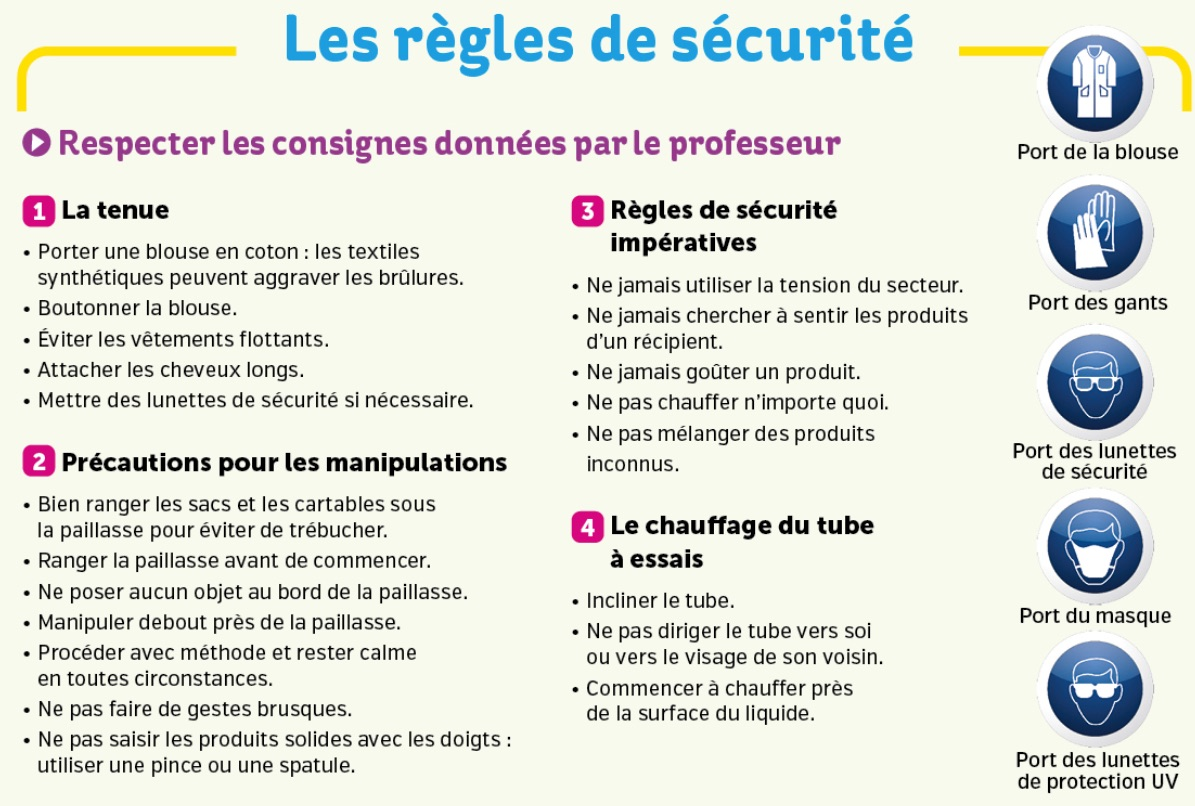
\includegraphics[width=0.8\linewidth]{securite.jpg}
  \label{Les règles de sécurité}
\end{figure}

\section{Identification des espèces chimiques}

\begin{figure}[H]
  \centering
  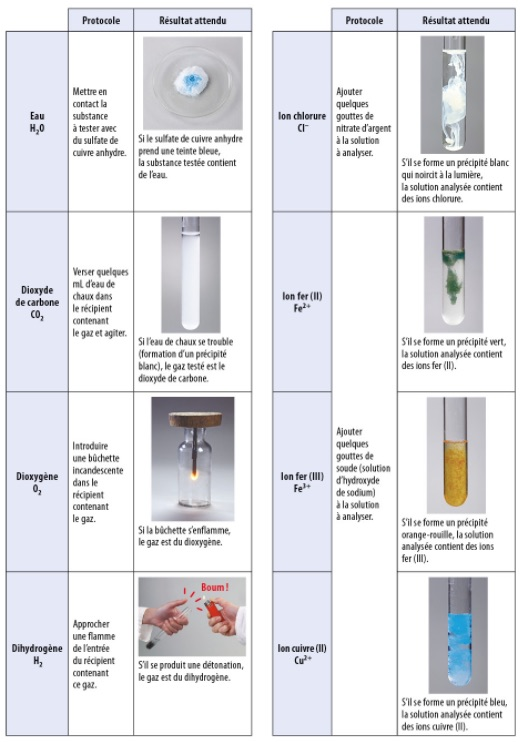
\includegraphics[width=0.9\linewidth]{identification.jpg}
  \label{Identification d'espèces chimiques}
\end{figure}

\end{document}
